%--------------------------------------------------------------------------------------------------%
\chapter{EVALUASI}
\label{chap:5}
%--------------------------------------------------------------------------------------------------%

Bab ini berisi evaluasi \textit{use case} KG yang dihasilkan oleh Lex2KG. Evaluasi yang akan
dilakukan adalah berupa SPARQL \textit{query} \textit{chat bot} sederhana, dan visualisasi \legal.
Alasan dari dilakukannya evaluasi kualitatif berupa \textit{use case evaluation} dibanding evaluasi
kuantitatif adalah karena penulis tidak menemukan metode evaluasi kuantitatif yang dapat dilakukan
dengan batasan lingkup penelitian. Sebagai contoh, untuk melakukan evaluasi kualitas KG yang
dihasilkan diperlukan \textit{gold standard} berupa KG yang dibuat oleh manusia dan dijamin benar,
kemudian diukur kualitasnya menggunakan suatu fungsi evaluasi. Membuat KG \textit{gold standard} ini
membutuhkan waktu yang lama, terutama pada kasus penelitian ini di mana ontologi KG nya juga
merupakan bagian penelitian dan dapat berubah dalam jangka waktu penelitian, yang artina
\textit{gold standard} nya juga dapat berubah-rubah.

%--------------------------------------------------------------------------------------------------%
\section{SPARQL Query}
\label{sec:sparq-query}
%--------------------------------------------------------------------------------------------------%

Dengan menggunakan SPARQL server seperi Apache Jena Fuseki, KG yang dibuat dengan Lex2KG dapat
dianalisis dengan menjalankan SPARQL \textit{query}. SPARQL \textit{query} memiliki fitur operasi
\textit{join}, \textit{union}, \textit{optional}, dan \textit{negation pattern}. SPARQL juga
menyediakan \textit{query} analisis yang lengkap seperti \textit{filter}, \textit{aggregate}, dan
\textit{property path}. Semua \textit{competency question} beserta SPARQL \textit{query} yang
menjawab pertanyaan tersebut terdapat pada lampiran. Pada subbab ini akan ditujukan sebaian dari
\textit{query} tersebut untuk dijelaskan fitur SPARQL dan ontologi KG yang digunakan.

%--------------------------------------------------------------------------------------------------%
\subsection{\textit{Query} Amendemen yang Dilakukan UU Cipta Kerja}
\label{subsec:cq8}
%--------------------------------------------------------------------------------------------------%
\textit{Competency question} No. 10 ``Tampilkan banyaknya penyisipan, pengubahan, dan penghapusan
pasal yang dilakukan UU Cipta Kerja terhadap UU lain.'' dapat dijawab dengan melakukan
\textit{query} \lst~\ref{lst:q-10} yang akan memberikan output \tab~\ref{tab:output-q-10}. Pada
\textit{query} digunakan properti \mono{o:menghapus}, \mono{o:menyisipkan}, dan \mono{o:mengubah}
untuk mencari \textit{triple} yang melakukan amendemen. Selain itu digunakan juga fitur SPARQL
\mono{UNION} untuk menggabungkan \textit{triple} dan \mono{BIND} untuk melakukan \textit{assignment}
variabel.

\begin{listing}[H]
  \begin{minted}[fontsize=\scriptsize, frame=single]{sparql}
PREFIX o: <https://example.org/lex2kg/ontology/>

SELECT ?type (COUNT(*) AS ?jumlah) WHERE {
  {
    ?point o:bagianDari+ <https://example.org/lex2kg/uu/2020/11> .
    ?point o:menghapus ?pasal .
    BIND("menghapus" AS ?type)
  } UNION {
    ?point o:bagianDari+ <https://example.org/lex2kg/uu/2020/11> .
    ?point o:menyisipkan ?pasal .
    BIND("menyisipkan" AS ?type)
  } UNION {
    ?point o:bagianDari+ <https://example.org/lex2kg/uu/2020/11> .
    ?point o:mengubah ?pasal .
    BIND("mengubah" AS ?type)
  }
} GROUP BY ?type
LIMIT 3
  \end{minted}
  \caption{SPARQL \textit{query} untuk \textit{competency question} No. 10}
  \label{lst:q-10}
\end{listing}

\begin{table}
  \centering
  \begin{tabular}{|l|r|} \hline
    \texttt{?type} & \texttt{?jumlah} \\\hline \hline
    "menyisipkan"  & 107              \\\hline
    "menghapus"    & 184              \\\hline
    "mengubah"     & 930              \\\hline
  \end{tabular}
  \caption{Output \textit{query} \lst~\ref{lst:q-10} }
  \label{tab:output-q-10}
\end{table}

%--------------------------------------------------------------------------------------------------%
\subsection{\textit{Query} Penimbangan pada Peraturan}
\label{subsec:cq15}
%--------------------------------------------------------------------------------------------------%

\textit{Competency question} No. 15 ``Tampilkan semua peraturan serta peraturan yang ditimbangnya.''
dapat dijawab dengan melakukan \textit{query} \lst~\ref{lst:q-15} yang akan memberikan output
\tab~\ref{tab:output-q-15}. Pada \textit{query} digunakan \mono{o:menimbang} untuk mencari entitas
``menimbang'', \mono{o:bagianDari*} untuk mendapatkan komponen dari entitas ``menimbang''. Selain itu
digunakan juga fitur SPARQL \mono{ORDER BY} yang pada kasus ini dugunakan untuk mengurutkan
\textit{triple} berdasarkan \mono{?penimbang} dan \mono{?ditimbang} secara \textit{descending}.


\begin{listing}[H]
  \begin{minted}[fontsize=\scriptsize, frame=single]{sparql}
PREFIX o: <https://example.org/lex2kg/ontology/>
PREFIX uu: <https://example.org/lex2kg/uu/>

SELECT ?penimbang ?ditimbang
WHERE {
  ?penimbang o:menimbang ?menimbang .
  ?menimbangText o:bagianDari* ?menimbang .
  ?menimbangText o:merujuk ?ditimbang .
  ?ditimbang a o:Peraturan
}
ORDER BY DESC(?penimbang) DESC(?ditimbang)
LIMIT 10

  \end{minted}
  \caption{SPARQL \textit{query} untuk \textit{competency question} No. 15}
  \label{lst:q-15}
\end{listing}

\begin{table}
  \centering
  \begin{tabular}{|l|l|} \hline
    \texttt{?penimbang} & \texttt{?ditimbang} \\\hline \hline
    \texttt{uu:2020/8}  & \texttt{uu:2018/12} \\\hline
    \texttt{uu:2020/6}  & \texttt{uu:2020/2}  \\\hline
    \texttt{uu:2020/6}  & \texttt{uu:2015/1}  \\\hline
    \texttt{uu:2020/6}  & \texttt{uu:2014/1}  \\\hline
    \texttt{uu:2020/2}  & \texttt{uu:2020/1}  \\\hline
  \end{tabular}
  \caption{Output \textit{query} \lst~\ref{lst:q-15} }
  \label{tab:output-q-15}
\end{table}

%--------------------------------------------------------------------------------------------------%
\subsection{\textit{Query} Banyaknya Amendemen Peraturan}
\label{subsec:cq20}
%--------------------------------------------------------------------------------------------------%

\textit{Competency question} No. 20 ``Tampilkan semua peraturan yang melakukan amendemen dan
banyaknya pasal yang amendemen oleh pasal tersebut.'' dapat dijawab dengan melakukan \textit{query}
\lst~\ref{lst:q-20} yang akan memberikan output \tab~\ref{tab:output-q-20}. Selain itu digunakan
juga fitur SPARQL \textit{property path} \mono{|} yang pada kasus ini predikat dapat berupa
\mono{o:mengubah}, \mono{o:menyisipkan}, atau \mono{o:menghapus}

\begin{listing}[H]
  \begin{minted}[fontsize=\scriptsize, frame=single]{sparql}
PREFIX o: <https://example.org/lex2kg/ontology/>
PREFIX uu: <https://example.org/lex2kg/uu/>

SELECT ?doc (COUNT(?point) as ?amendmentCount)
WHERE {
  ?doc a o:Peraturan .
  ?point o:bagianDari* ?doc .
  ?point o:mengubah|o:menyisipkan|o:menghapus ?pasalVersion .
}
GROUP BY (?doc)
ORDER BY DESC(?amendmentCount)
LIMIT 10
  \end{minted}
  \caption{SPARQL \textit{query} untuk \textit{competency question} No. 20}
  \label{lst:q-20}
\end{listing}

\begin{table}
  \centering
  \begin{tabular}{|l|r|} \hline
    \texttt{?doc}       & \texttt{?amandementCount} \\\hline \hline
    \texttt{uu:2020/11} & 1221                      \\\hline
    \texttt{uu:2011/8}  & 20                        \\\hline
    \texttt{uu:2009/26} & 11                        \\\hline
  \end{tabular}
  \caption{Output \textit{query} \lst~\ref{lst:q-20} }
  \label{tab:output-q-20}
\end{table}

%--------------------------------------------------------------------------------------------------%
\section{Visualisasi KG}
\label{sec:visualisasi-kg}
%--------------------------------------------------------------------------------------------------%

Visualisasi data dapat meningkatkan visibilitas dan \textit{explainability} KG. Pada KG dapat
dilakukan visualisasi \textit{node} dan \textit{relation} antara \textit{node}, atau visualisasi
statistik dari KG tersebut. Pada Subbab ini akan diberikan beberapa contoh visualisasi menggunakan
\textit{library} visualisasi VizKG.\footnote{\url{https://pypi.org/project/VizKG/}}

%--------------------------------------------------------------------------------------------------%
\subsection{\textit{Word Cloud} UU Ketenagakerjaan}
\label{subsec:word-cloud}
%--------------------------------------------------------------------------------------------------%

\lst~\ref{lst:vizkg1} merupakan kode untuk melakukan visualisasi \textit{word cloud} dari UU 13/2003
tentang Ketenagakerjaan. Teks yang digunakan untuk \textit{word cloud} diambil dari teks-teks yang
terdapat pada UU 13/2003. Hasil visualisasi pada \pic~\ref{fig:vizkg1} menunjukan bahwa UU ini
paling banyak membicarakan tentang pekerja buruh dan perjanjian kerja.

\begin{listing}[H]
  \begin{minted}[fontsize=\scriptsize, frame=single, breaklines]{python}
sparql_query = """
PREFIX o: <https://example.org/lex2kg/ontology/>
SELECT* WHERE { 
?komponen o:bagianDari* <https://example.org/lex2kg/uu/2003/13> ;
          a o:Segmen ;
          o:teks ?teks .
}
"""
words = vkg(sparql_query=sparql_query, sparql_service_url=sparql_service_url, chart='WordCloud')
words.plot()
  \end{minted}
  \caption{Visualisasi ``Tampilkan 5 peraturan dengan komponen terbanyak beserta jumlah komponennya'' menggunakan VizKG}
  \label{lst:vizkg1}
\end{listing}

\begin{figure}[H]
  \centering
  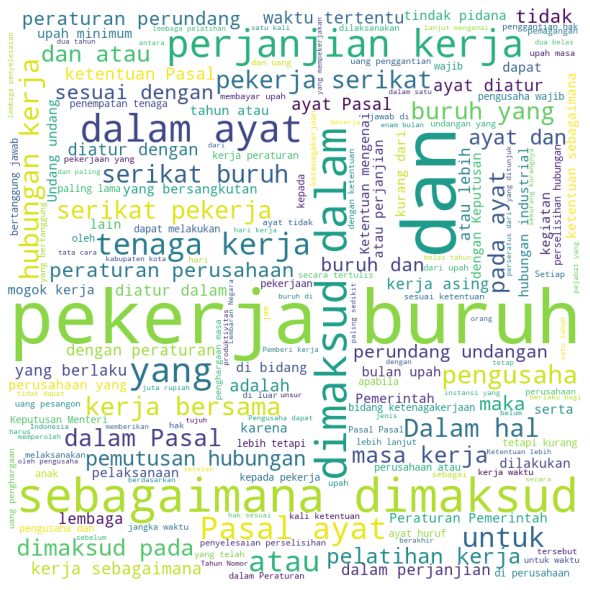
\includegraphics[scale=0.5]{pictures/vizkg1.png}
  \caption{Output VizKG untuk \lst~\ref{lst:vizkg1}}
  \label{fig:vizkg1}
\end{figure}

%--------------------------------------------------------------------------------------------------%
\subsection{Diagram Garis Jumlah UU per Tahun}
\label{subsec:diagram-garis}
%--------------------------------------------------------------------------------------------------%

\lst~\ref{lst:vizkg2} merupakan kode untuk melakukan visualisasi diagram garis jumlah undang-undang
setiap tahunnya. Hasil visualisasi pada \pic~\ref{fig:vizkg2} menunjukan jumlah UU setiap tahunnya
cenderung bertambah. Perlu diperhatikan bahwa UU yang terdapat pada KG hanya UU yang berhasil
dikonversi oleh Lex2KG, oleh sebab itu kecenderungan penambahan jumlah UU bisa jadi disebabkan oleh
kualitas PDF yang makin baik setiap tahunnya.

\begin{listing}[H]
  \begin{minted}[fontsize=\scriptsize, frame=single, breaklines]{python}
sparql_query = """
PREFIX o: <https://example.org/lex2kg/ontology/>
SELECT ?tahun (COUNT(?peraturan) as ?peraturanCount)
WHERE { ?peraturan o:tahun ?tahun .}
GROUP BY ?tahun
ORDER BY ?tahun
"""
words = vkg(sparql_query=sparql_query, sparql_service_url=sparql_service_url, chart='linechart')
words.plot()
  \end{minted}
  \caption{Visualisasi ``Tampilkan 5 peraturan dengan komponen terbanyak beserta jumlah komponennya'' menggunakan VizKG}
  \label{lst:vizkg2}
\end{listing}

\begin{figure}[H]
  \centering
  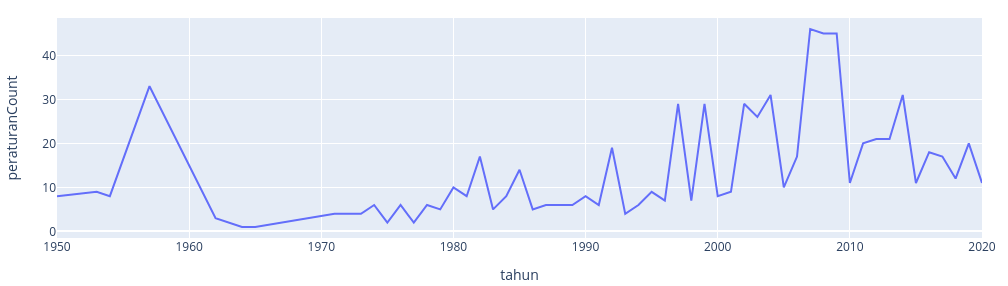
\includegraphics[width=\textwidth]{pictures/vizkg2.png}
  \caption{Output VizKG untuk \lst~\ref{lst:vizkg2}}
  \label{fig:vizkg2}
\end{figure}

%--------------------------------------------------------------------------------------------------%
\subsection{\textit{Graph} ``menimbang''}
\label{subsec:graph}
%--------------------------------------------------------------------------------------------------%

\lst~\ref{lst:vizkg3} merupakan kode untuk melakukan visualisasi \textit{graph} yang menunjukan
hubungan \mono{o:menimbang} antara peraturan, di mana peraturan penimbang disahkan setelah tahun
2017. Hasil visualisasi pada \pic~\ref{fig:vizkg3} bahwa tidak jarang sebuah peraturan ditimbang
oleh atau menimbang lebih dari satu peraturan. Peraturan yang paling banyak ditimbang oleh UU
setelah tahun 2017 adalah UU 24/2000 tentang Perjanjian Internasional.

\begin{listing}[H]
  \begin{minted}[fontsize=\scriptsize, frame=single, breaklines]{python}
sparql_query = """
PREFIX o: <https://example.org/lex2kg/ontology/>
PREFIX uu: <https://example.org/lex2kg/uu/>

SELECT DISTINCT ?penimbang ?penimbangStr ?ditimbang ?ditimbangStr
WHERE {
  ?penimbang o:menimbang ?menimbang .
  ?menimbangText o:bagianDari* ?menimbang .
  ?menimbangText o:merujuk ?ditimbang .
  ?ditimbang a o:Peraturan .
  ?penimbang o:tahun ?tahun .
  BIND(REPLACE(STR(?penimbang),"https://example.org/lex2kg/","") as ?penimbangStr) .
  BIND(REPLACE(STR(?ditimbang),"https://example.org/lex2kg/","") as ?ditimbangStr) .
  FILTER(?tahun > 2017)
}
"""
graph = vkg(sparql_query=sparql_query, sparql_service_url=sparql_service_url, chart="graph")
graph.plot()
  \end{minted}
  \caption{Visualisasi ``Tampilkan 5 peraturan dengan komponen terbanyak beserta jumlah komponennya'' menggunakan VizKG}
  \label{lst:vizkg3}
\end{listing}

\begin{figure}[H]
  \centering
  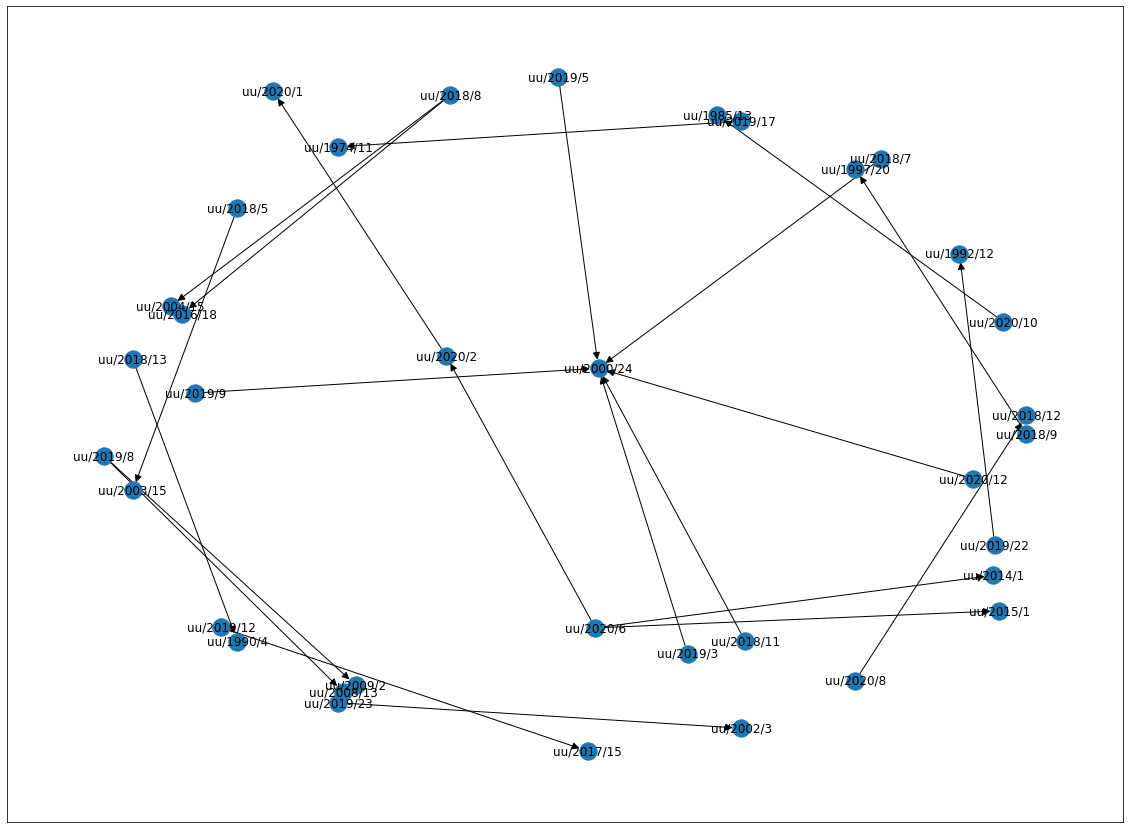
\includegraphics[width=\textwidth]{pictures/vizkg3.png}
  \caption{Output VizKG untuk \lst~\ref{lst:vizkg3}}
  \label{fig:vizkg3}
\end{figure}


%--------------------------------------------------------------------------------------------------%
\section{\textit{Chat bot} sederhana}
\label{sec:chatbot-sederhana}
%--------------------------------------------------------------------------------------------------%

% // HACK: tmbhkn satu skenario yg smpai liat konten

KG \legal dapat digunakan pada \textit{chat bot}. \textit{Chat bot} sederhana memberikan pertanyaan
yang sudah disediakan dan mengembalikan jawaban berdasarkan input pengguna sesuai program
deterministik yang diimplementasi. Pada bab ini akan diperlihatkan bagaimana pengguna melalui
beberapa skenario dan bagaimana \textit{chat bot} nya bekerja. Skenario \textit{chatbot} adalah
sekuensial, artinya Skenario 2 adalah lanjutan dari Skenario 1, dan Skenario 3 adalah lanjutan dari
Skenario 2. Input pengguna akan digunakan sebagai input dari template SPARQL \textit{query} yang
sudah tersedia. Teks yang ditampilkan \textit{chat bot} ditandai dengan warna hitam, dan teks input
pengguna ditandai dengan \textcolor{red}{warna merah}.

%--------------------------------------------------------------------------------------------------%
\subsection{Skenario 1: Mencari Peraturan dengan Kata Kunci}
\label{subsec:skenario-1}
%--------------------------------------------------------------------------------------------------%

\lst~\ref{lst:chatbot-1} merupakan tampilan chatbot pada Skenario 1 di mana pengguna dapat mencari
\legal dengan kata kunci tertentu. Pada contoh ini pengguna mencari peraturan dengan kata kunci
``kerja'', kemudian \textit{chat bot} melakukan \textit{query} terhadap KG menggunakan template
\lst~\ref{lst:chatbot-1-query}, di mana \mono{inputStr} memiliki nilai ``kerja''. Kemudian
\textit{chat bot} mengembalikan hasil \textit{query} berupa nama \legal yang pada judulnya terdapa
\textit{substring} kerja.

\begin{listing}[H]
  \begin{center}
    \begin{tabular}{|p{0.9\textwidth}|}
      \hline
      \makecell[l]{
        \texttt{Masukkan Kata Kunci Peraturan: \textcolor{red}{kerja}}    \\ \\
        \texttt{Berikut adalah peraturan yang judulnya mengandung kerja.} \\
        \texttt{Pilih salah satu untuk melihat lebih lanjut.}             \\
        \texttt{uu/2004/17}                                               \\
        \texttt{uu/2016/3}                                                \\
        \texttt{uu/1997/25}                                               \\
        \texttt{uu/2016/15}                                               \\
        \texttt{uu/2007/47}                                               \\
        \texttt{uu/1991/1}                                                \\
        \texttt{uu/2019/3}                                                \\ \\
        \texttt{Pilih salah satu untuk melihat lebih lanjut: }
      }                                                                   \\
      \hline
    \end{tabular}
  \end{center}
  \caption{Tampilan \textit{chat bot} untuk Skenario 1}
  \label{lst:chatbot-1}
\end{listing}

\begin{listing}[H]
  \begin{minted}[fontsize=\scriptsize, frame=single]{typescript}
    const res = await sparqlQuery({
      queryStr: `
PREFIX o: <https://example.org/lex2kg/ontology/>
SELECT ?doc ?title
WHERE {
  ?doc a o:Peraturan .
  ?doc o:tentang ?title.
  FILTER REGEX(STR(?title), "${inputStr.toUpperCase()}")
}
`,
    });
  \end{minted}
  \caption{\textit{Query} template untuk Skenario 1}
  \label{lst:chatbot-1-query}
\end{listing}

%--------------------------------------------------------------------------------------------------%
\subsection{Skenario 2: Menampilkan Metadata Peraturan}
\label{subsec:skenario-2}
%--------------------------------------------------------------------------------------------------%

\lst~\ref{lst:chatbot-2} merupakan tampilan chatbot pada Skenario 2 di mana pengguna memilih
peraturan berdasarkan pilihan yang diberikan sebelumnya, kemudian menampilkan metadatanya. Pada
contoh ini pengguna memilih peraturan \mono{uu/2019/3} dan data\mono{metadata}, kemudian
\textit{chat bot} melakukan \textit{query} terhadap KG menggunakan template
\lst~\ref{lst:chatbot-2-query}, di mana \mono{legalURI} memiliki nilai \mono{uu/2019/3}. Kemudian
\textit{chat bot} mengembalikan hasil \textit{query} berupa metadata UU 3/2019.

\begin{listing}[H]
  \begin{center}
    \begin{tabular}{|p{0.9\textwidth}|}
      \hline
      \makecell[l]{
        \texttt{Pilih salah satu untuk melihat lebih lanjut: \textcolor{red}{uu/2019/3}} \\
        \\
        \texttt{Data uu/2019/3 :}                                                        \\
        \texttt{-metadata}                                                               \\
        \texttt{-menimbang}                                                              \\
        \texttt{-konten}                                                                 \\
        \\
        \texttt{Pilih data yang ingin anda lihat: \textcolor{red}{metadata}}             \\
        \\
        \texttt{yurisdiksi: Indonesia}                                                   \\
        \texttt{jenisPeraturan: UU}                                                      \\
        \texttt{tahun: 2019}                                                             \\
        \texttt{bahasa: id}                                                              \\
        \texttt{tentang:  PENGESAHAN NOTA KESEPAHAMAN ANTARA PEMERINTAH REPUBLIK...}     \\
        \texttt{disahkanPada: 2009-01-10}                                                \\
        \texttt{disahkanDi: Jakarta}                                                     \\
        \texttt{disahkanOleh: JOKO WIDODO}                                               \\
        \texttt{jabatanPengesah: PRESIDEN REPUBLIK INDONESIA,}                           \\
        \\
        \texttt{Pilih data yang ingin anda lihat:}
      }                                                                                  \\
      \hline
    \end{tabular}
  \end{center}
  \caption{Tampilan \textit{chat bot} untuk Skenario 2}
  \label{lst:chatbot-2}
\end{listing}



\begin{listing}[H]
  \begin{minted}[fontsize=\scriptsize, frame=single, breaklines]{typescript}
    const res = await sparqlQuery({
      queryStr: `
PREFIX o: <https://example.org/lex2kg/ontology/>
SELECT ?label ?data
WHERE {
<https://example.org/lex2kg/${legalURI}> o:yurisdiksi| o:jenisPeraturan| o:tahun| o:bahasa| o:tentang| o:disahkanPada| o:disahkanDi| o:disahkanOleh| o:jabatanPengesah ?data ;
    ?label ?data .
}
`,
    });
  \end{minted}
  \caption{\textit{Query} template untuk Skenario 2}
  \label{lst:chatbot-2-query}
\end{listing}

%--------------------------------------------------------------------------------------------------%
\subsection{Skenario 3: Melihat Peraturan yang ditimbang oleh Peraturan}
\label{subsec:skenario-3}
%--------------------------------------------------------------------------------------------------%

\lst~\ref{lst:chatbot-3} merupakan tampilan chatbot pada Skenario 3 di mana pengguna memilih
peraturan berdasarkan pilihan yang diberikan sebelumnya, kemudian menampilkan peraturan yang
ditimbangnya. Pada contoh ini pengguna memilih \mono{menimbang} untuk informasi yang ingin
ditampilkan, kemudian \textit{chat bot} melakukan \textit{query} terhadap KG menggunakan template
\lst~\ref{lst:chatbot-3-query}, di mana \mono{legalURI} memiliki nilai \mono{uu/2019/3}. Kemudian
\textit{chat bot} mengembalikan hasil \textit{query} berupa dokumen yang ditimbang UU 3/2019 yaitu
UU 24/2000.

\begin{listing}[H]
  \begin{center}
    \begin{tabular}{|p{0.9\textwidth}|}
      \hline
      \makecell[l]{
        \texttt{Data uu/2019/3 :}                                             \\
        \texttt{-metadata}                                                    \\
        \texttt{-menimbang}                                                   \\
        \texttt{-konten}                                                      \\
        \\
        \texttt{Pilih data yang ingin anda lihat: \textcolor{red}{menimbang}} \\
        \\
        \texttt{uu/2000/24}
      }                                                                       \\
      \hline
    \end{tabular}
  \end{center}
  \caption{Tampilan \textit{chat bot} untuk Skenario 3}
  \label{lst:chatbot-3}
\end{listing}

\begin{listing}[H]
  \begin{minted}[fontsize=\scriptsize, frame=single, breaklines]{typescript}
    const res = await sparqlQuery({
      queryStr: `
PREFIX o: <https://example.org/lex2kg/ontology/>
SELECT DISTINCT ?ditimbang
WHERE {
  <https://example.org/lex2kg/${legalURI}> o:menimbang ?menimbang .
  ?menimbangText o:bagianDari* ?menimbang .
  ?menimbangText o:merujuk ?ditimbang .
}
`,
    });
  \end{minted}
  \caption{\textit{Query} template untuk Skenario 3}
  \label{lst:chatbot-3-query}
\end{listing}

%--------------------------------------------------------------------------------------------------%
\subsection{Skenario 4: Melihat Konten Peraturan}
\label{subsec:skenario-4}
%--------------------------------------------------------------------------------------------------%

\lst~\ref{lst:chatbot-4} merupakan tampilan chatbot pada Skenario 4 di mana pengguna memilih
peraturan berdasarkan pilihan yang diberikan sebelumnya, kemudian menampilkan konten teks dari
peraturan tersebut. Pada contoh ini pengguna memilih \mono{konten} untuk informasi yang ingin
ditampilkan. \textit{Chat bot} melakukan \textit{query} terhadap KG menggunakan template
\lst~\ref{lst:chatbot-4-1-query} untuk mengetahui banyaknya pasal pada UU 3/2019. Setelah mengetahui
banyaknya pasal, pengguna meilih untuk menampilkan pasal 2. Kemudian \textit{Chat bot} melakukan query
menggunakan template \lst~\ref{lst:chatbot-4-2-query} untuk mendapatkan teks dari pasal 2, di mana
\mono{noPasal} pada template diisi nilai "2".

\begin{listing}[H]
  \begin{center}
    \begin{tabular}{|p{0.9\textwidth}|}
      \hline
      \makecell[l]{
        \texttt{Data uu/2019/3 :}                                          \\
        \texttt{-metadata}                                                 \\
        \texttt{-menimbang}                                                \\
        \texttt{-konten}                                                   \\
        \\
        \texttt{Pilih data yang ingin anda lihat: \textcolor{red}{konten}} \\
        \\
        \texttt{Pilih nomor pasal [1-2]: \textcolor{red}{2}}               \\
        \\
        \texttt{Konten Pasal 2 UU 3/2019:}                                 \\
        \texttt{(1). Mengesahkan Nota Kesepahaman antara }                 \\
        \texttt{Pemerintah Republik Indonesia dan Pemerintah}              \\
        \texttt{Republik Serbia tentang Kerja Sama di Bidang...}           \\
      }                                                                    \\
      \hline
    \end{tabular}
  \end{center}
  \caption{Tampilan \textit{chat bot} untuk Skenario 4}
  \label{lst:chatbot-4}
\end{listing}

\begin{listing}[H]
  \begin{minted}[fontsize=\scriptsize, frame=single, breaklines]{typescript}
    const res = await sparqlQuery({
      queryStr: `
PREFIX o: <https://example.org/lex2kg/ontology/>

SELECT (COUNT(?pasal) as ?pasalCount)
WHERE {
  ?pasal o:bagianDari+ <https://example.org/lex2kg/${legalURI}>;
         a o:Pasal.
}
`,
    });
  \end{minted}
  \caption{\textit{Query} template pada Skenario 4 untuk menghitung jumlah pasal pada UU 3/2019}
  \label{lst:chatbot-4-1-query}
\end{listing}

\begin{listing}[H]
  \begin{minted}[fontsize=\scriptsize, frame=single, breaklines]{typescript}
    const res = await sparqlQuery({
      queryStr: `
PREFIX o: <https://example.org/lex2kg/ontology/>

SELECT DISTINCT ?teks
WHERE {
  ?pasal o:bagianDari+ <https://example.org/lex2kg/${legalURI}>;
            a o:Pasal;
            o:nomor ${noPasal} .
  ?komponen o:bagianDari* ?pasal;
            o:teks ?teks.
}
ORDER BY ?komponen
`,
    });
  \end{minted}
  \caption{\textit{Query} template pada Skenario 4 untuk menampilkan teks pasal 2 UU 3/2019}
  \label{lst:chatbot-4-2-query}
\end{listing}

